%\documentclass[3p]{elsarticle}
\documentclass[5p]{elsarticle}
\usepackage{epstopdf}
\epstopdfsetup{outdir=./}
\DeclareGraphicsRule{.eps}{pdf}{.pdf}{`epstopdf #1}
\usepackage{natbib,graphicx,amsmath, mhchem,url,colortbl,fancyhdr,subfigure}
\usepackage{multicol}


\journal{EECS 545}
\providecommand{\e}[1]{\ensuremath{\times 10^{#1}}}

\newcolumntype{L}[1]{>{\raggedright\let\newline\\\arraybackslash\hspace{0pt}}m{#1}}

\begin{document}
\begin{frontmatter}

%\input{header.tex}
\title{Methods for Polyphonic Music Transcription} % Remove Piano part?
% 'Everything you wanted to know about polyphonic music transcription'
% Note: according to Scott's final report list, it looks like the best paper according to him is a really thorough survey of an already established field, and he repeatedly indicates that he doesn't necessarily expect any new methods
\author[eadd]{Jeremy Nash}
\ead{nashj@umich.edu}
\author[eadd]{Paul Schroeder}
\ead{pschro@umich.edu}
\address[eadd]{Electrical Engineering Department, University of Michigan, Ann Arbor, MI 48109}
\author[csadd]{Mark Liu}
\ead{markmliu@umich.edu}
\address[csadd]{Computer Science Department, University of Michigan, Ann Arbor, MI 48109}


% Pictures to add to paper:
% spectrogram of single note
% spectrogram of multiple notes

% Show FFT vs. Constant q or log bins

% Show SVM output
% Show SVM with HMM output

% Show NMF output and NMF output with sparsity constraint
% Show NMF with Itakura-Saito Divergence





%\input{abstract.tex}

\begin{abstract}
% 4 sentences - write this last

% State the problem
%We present a review of modern methods for polyphonic music transcription.

Music transcription is the process of converting an audio recording into a musical score.
Musicians have been transcribing music manually for centuries to learn new songs and gain musical insight.
Transcription, however, is an arduous manual process for musicians, and it's a difficult problem for computers because the pitches in a musical score are the human perceptions of a time-varying and frequency-varying physical phenomenon.
There has been a flurry of research on how to solve this problem.
We investigate the best solutions to the automated transcription problem and evaluate and compare their performance.



% Say why it's an interesting problem

% Say what your solution achieves

% Say what follows from your solution


\end{abstract}
\begin{keyword}
Transcription \sep sparse coding \sep non-negative matrix factorization \sep Bayesian non-parametrics \sep music information retrieval
\end{keyword}

\end{frontmatter}

\setcounter{topnumber}{1}

\section{Introduction}


\subsection{Terminology}
Semitones are the smallest music interval in Western music. On a piano, semitones are the adjacent keys.

Timbre represents the spectral envelope, time envelope, noise, tonality, and onset of a musical note. Timbre captures the unique properties of a musical instrument.

Pitches are represented by the notes used in musical notation. Pitches are a psychological perception and not an objective physical property. While we can intuitively assign a linear order to pitches (by referring to pitches as lower or higher than other pitches), pitches are rarely a single frequency and are instead a function of their timbre.

Polyphony means multiple simultaneous notes. Monophony means only a single note at a time. These terms carry slightly different meanings outside of automated transcription research.

\section{Motivation}
% No more than one page

% Introduction

% Explain motivation

% This is just copied from 'A Connectionist Approach to Automatic Transcription of Polyphonic Piano Music' for now:
Music transcription is the process of creating a musical score from an audio recording.  There are many applications of music transcription. Transcription produces a compact and standardized parametric representation of music, which is necessary for content-based retrieval of music in most current musical databases. It is also useful in music analysis systems for tasks such as melody extraction, music segmentation and rhythm tracking. Transcription aids musicologists in analyzing music that has never been written down, such as improvised or ethnical music. The conversion of an acoustical waveform into parametric description is also useful in the process of making music, as well as in newer coding standards, such as MPEG-4, which may include such descriptions.

Historically, the task of music transcription has been left to expert musicians.  However, the process is difficult and time-consuming for complex recordings.  Thus the ability to automatically transcribe music is of both practical and theoretical interest.


% According to Simon Peyton Jones:
% Here is a problem
% It's an interesting problem
% It's an unsolved problem
% Here is my idea
% My idea works
% Here's how my idea compares to other approaches


% Describe the problem
%    Use an example to introduce the problem
% State your contributions
%    Bulleted list of contributions


% Explain like you're at a whiteboard

% Here's why people want to do this
% Study of music - understanding music
% recommender systems
% Music information database
% For learning musicians

% Here's why it's difficult
% Musical timbres
% Time varying - attack, decay, sustain, release
% Number of sources?
% Human perception of pitch
% Musical instrument tuning
% Completely new instruments - software created


% Here's a teaser on how I'm going to solve this problem

% Here's what I'm about to show you




\section{Problem Statement}
% No more than one page

In Western music, each note corresponds to a single, fundamental frequency. The musical note A above middle C corresponds to 440Hz. If this were the complete story, there would be a one-to-one correspondence between frequencies and notes, and the transcription problem would be as simple as converting the frequencies into notes. The reality, however, is that each instrument has a unique timbre with a set of overtones that vary over time and overlap with the frequencies of other notes.

Like most research in automatic music transcription, we restrict our problem to transcribing polyphonic piano music. The reason for this is primarily the availability of online piano MIDI databases and the popularity of the piano in Western music. At the same time, the piano has a complex timbre and adequately represents the difficulties in the generic transcription problem.

\subsection{Piano physics}

The physical description of sound production in a piano is complex. \citet{bank2003physically} describes physics-based synthesis algorithm that models the piano hammer as a nonlinear spring connect to a lumped mass, a nonideal, lossy piano string with digital waveguides, and soundboard radiation with a linear filter. This model gives rise to the rich and variable set of overtones across the keyboard. Furthermore, in a procedure called stretched tuning, real pianos have their higher notes tuned slightly higher and their lower notes tuned slightly lower to compensate for psychoacoustic detuning effect in our ears. These factors give rise to the complex spectral feature space for our machine learning methods.

% \section{Related Work}
% Contain a table with metrics data, brief description, year published


\section{Methodologies}
There are currently two main approaches to polyphonic music transcription. The first approach learns a supervised learning model that uses frequency magnitudes to predict the presence of a note. The second approach uses unsupervised learning techniques to simultaneously extract notes and a musical score from a spectrogram. The following sections detail the most popular techniques within these general approaches.

\subsection{Audio data}
Our training data comes from a large database of piano MIDI files. MIDI is a standard for specifying the controlling and playing of digital instruments. A MIDI specifies the instruments, notes, volumes and the other information needed to digitally synthesize(sp?) a song. MIDI files may specify a type of instrument but the exact sonic characteristics of the virtual instrument are defined by the synthesizer. That is, two identical midi files played with different sythnesizers may sound different.

MIDI is an eminently useful technology for the development of transcription technology. It contains both the time-coded note information and is capable of producing the corresponding audio file, which are respectively the output and input of the transcription system. Having raw audio and note information that are time-aligned is important as the note information can act as the labels in supervised learning.

Digital audio can be stored using WAV files. WAV files are uncompressed and directly store digital audio samples. A typical WAV file is at CD quality: 16 bit samples at 44.1 KSa/s. We found that many transcription techniques downsample the audio (e.g. to 8 or 16 KSa/s) before processing, with the idea being that the higher frequency information lost in downsampling is not useful for transcription and that transcription is faster with fewer samples to process \citet{}.
%musical score
%While MIDI specifies the type of instrument,
% MIDI instrument not specified in the file
%a standard for specifying

%Wav files are...

%44.1kHz

%16kHz sampling rate, 16 bit,
%Databases

% Sampling rate for piano

% STFT
\subsection{Spectrogram}
% Hint at the matrix factorization approach

In all of the methods we explored, we computed a spectrogram of the wav file with a window size of 128ms, a Hanning windowing function, and a 10ms hop between frames. This window size gives us a frequency resolution of 8Hz, which is slightly inadequate for resolving the fundamental frequencies of lower notes and overly resolute for the higher frequencies due to the logarithmic spacing of the semitone fundamental frequencies.

To the authors' knowledge, all of the methods in the transcription literature compute a spectrogram as a preprocessing step before applying their specialized algorithm. In the NMF methods, the spectrogram matrix is decomposed into a piano roll matrix and the note spectrum dictionary matrix. In the supervised classifier methods, the classifiers use features from the spectrogram matrix to predict the presence of a note.


\begin{figure*}[t]
\begin{center}
\subfigure[]{
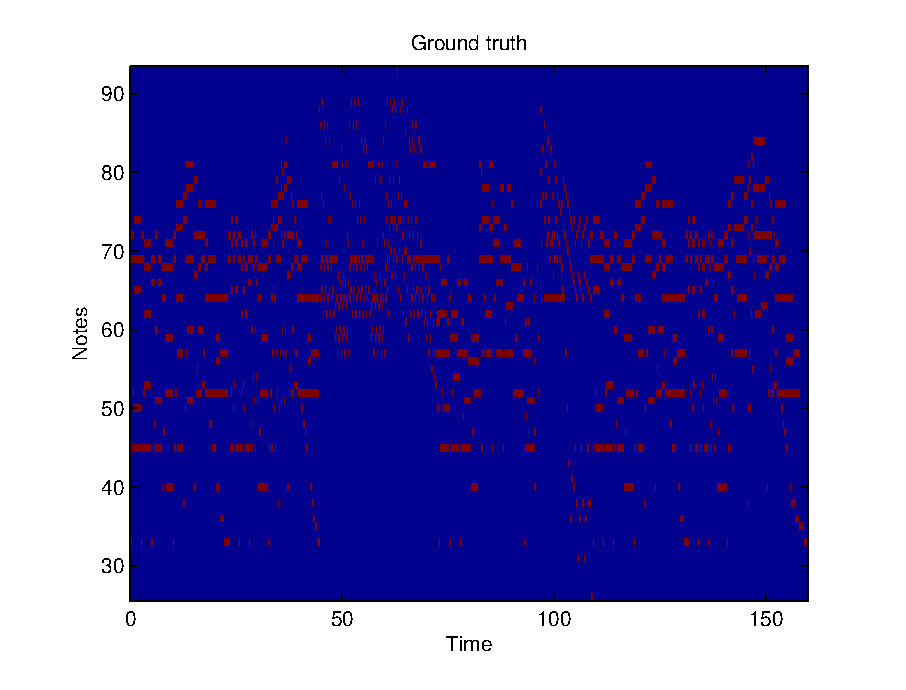
\includegraphics[scale=.6]{pianorollsong}
\label{fig:pianorollsong}
}
\subfigure[]{
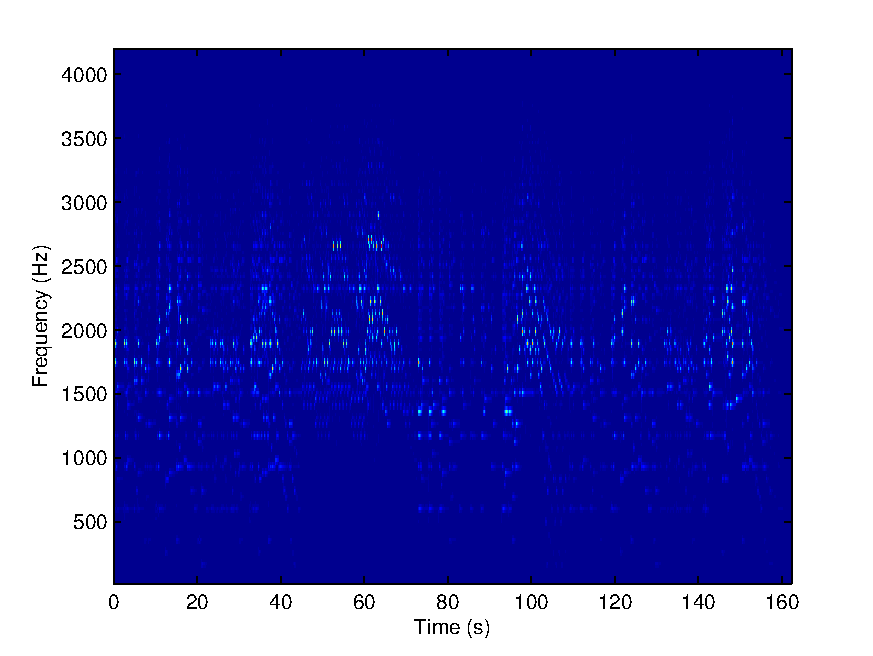
\includegraphics[scale=.6]{brim2ud}
\label{fig:brim2ud}
}
\end{center}
\caption{(a) shows the piano roll generated from a MIDI file. (b) shows a spectrogram of the wav file using the constant Q transform with a step size of 10ms. One can immediately see the similarity in the shape of the two plots, although the transcription process is complicated by the overlapping frequencies, changing volume, and noise in the spectrogram plot.}
\end{figure*}

\subsection{Constant Q transform}
Unlike the linear frequency scale used in an FFT, semitones in Western music are spaced logarithmically. This logarithmic spacing derives from our roughly logarithmic perception of pitches, first captured by \citet{stevens1937scale} through the mel scale.

Transforming the spectra to a logarithmic frequency scale achieves two main benefits. It reduces the dimensionality of the training data, since most of the spectral energy occupies a logarithmic grid of frequencies. In practice, \citet{bock2012polyphonic} were able to reduce the dimensionality of their training data from 2048 FFT magnitudes down to 183.

The logarithmic frequency scale also decreases sensitivty to detuning. In a linear frequency scale, detuning, especially in higher semitones, will cause spectral energy to leak into neighboring frequency bins, creating more variability in the training data. On a logarithmic frequency scale, minor detuning would result in less spectral energy leakage and less unnecessary variability in the training data.

\subsection{Note onset detection}
This method proposes restricting the problem to determining note onsets. This is a simpler problem than detecting note durations because of the possibility for time-varying timbres in instruments. Many researchers in this field evaluate their music transcription methods on their note onset detection performance. In this paper, we chose to evaluate our methods over the entire duration of the notes; while this brings us closer to the original musical score, it also results in higher error measures.

\subsection{Discriminative models}
% SVM, logistic regression
Applying discriminative machine learning models to detect notes is a dominant approach in transcription research. A discriminative model can be learned for each note (for pianos, 88 classifiers) over the frequency magnitudes of the song's spectrogram. Each note classifier outputs whether the note is present or absent at each time step determined by the time step used in the spectrogram. Many researchers have chosen nonlinear or kernel-based methods due to the complexity of the input space.

\subsection{SVM}



% use support vector machines to predict note presence or absence at 10ms time steps based on
\citet{poliner2006discriminative} first used short-time Fourier transforms were applied to the audio data.  Then,  87(they omit the highest note) one-versus-all (OVA) SVM classifiers were trained, one for each note.  The SVM's were then used to predict the test data, and HMM's were used for post-process smoothing.
% one vs all
% frequency partition

\subsection{Restricted Boltzmann machine}

To increase the previous system's robustness to noise, \citet{nam2011classification} proposed a preprocessing stage using a restricted Boltzmann machine on the spectrogram features. The RBM would be able to learn noise invariant features over the spectrogram and provide a new input to the SVM classifiers. The researchers found a modest improvement in performance as they increased noise levels in their input data.

\subsection{Boosted classifier}

\citet{boogaart2009note} proposes using AdaBoost with decision stumps for the weak learners to detect note onsets. The motivation for using AdaBoost in transcription over other methods is its robustness to overfitting the spectral features and its interpretability in the transcription process. The interpretation is that the decision stumps decide on the presence of a note based on the magnitudes of the fundamental frequency of a note and then its overtones. In some sense, this is a more sophisticated version of applying a threshold to the constant Q transform, but it suffers from the same problems; the method has difficulty with volume changes in the song, and dense chords with many overlapping overtones can also confuse the decision stumps.

% \subsection{Feed forward neural network}

\begin{figure*}[t]
\begin{center}
\subfigure[]{
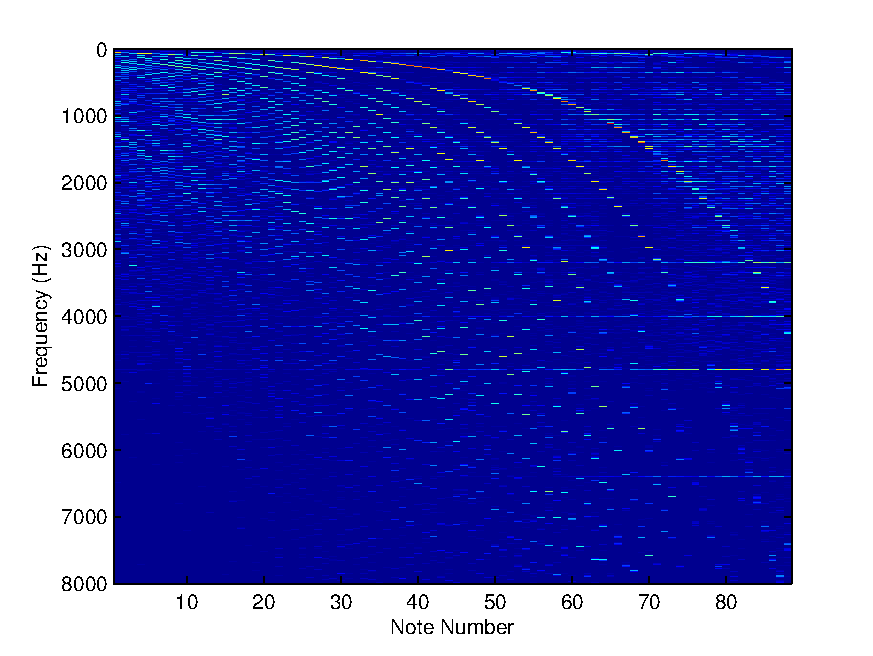
\includegraphics[scale=.6]{stft-dictionary}
\label{fig:stftdict}
}
\subfigure[]{
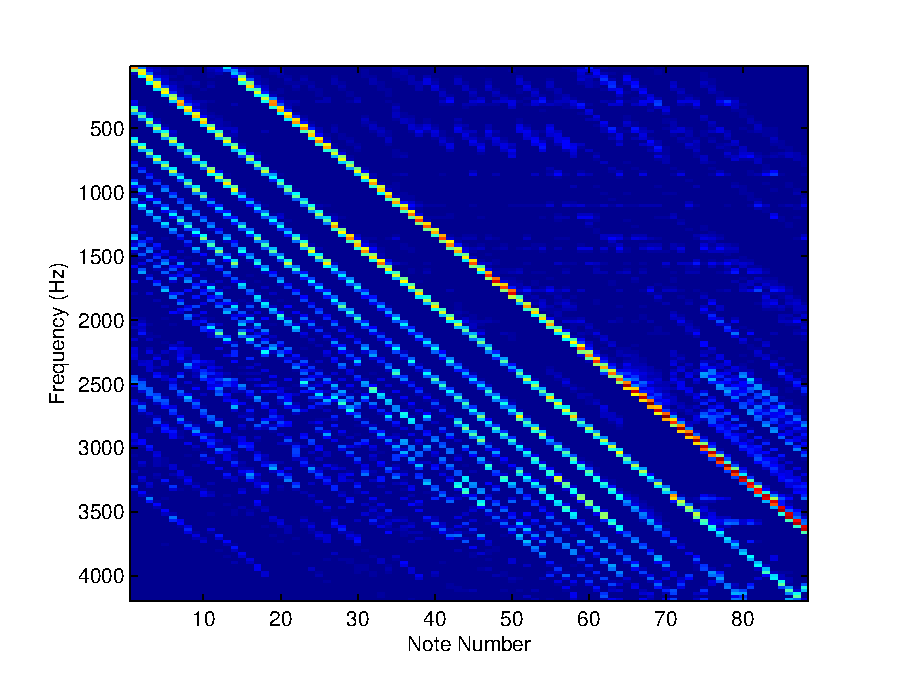
\includegraphics[scale=.6]{cqt-dictionary}
\label{fig:cqtdict}
}
\end{center}
\caption{ Two W dictionary matrices computed for the supervised NMF method. Each column represents the spectral signature of a piano note. (a) The W dictionary matrix computed using an STFT. (b) The W dictionary matrix computed using constant Q transform.}
\end{figure*}

\subsection{Non-negative matrix factorization}

Non-negative matrix factorization (NMF) is an unsupervised, dimensionality reduction technique that factors a non-negative matrix $V$ with dimensions $F \times N$ into two non-negative matrices $W$ and $H$.

\[ V \approx WH \]

\noindent where $W$ is an $F \times K$ matrix and $H$ is a $K \times N$ matrix. $K$ is typically chosen so that $F*K + K*N << F*N$.

Typically this factorization is performmed with the goal of recovering some useful structure or information from the matrix factors. NMF has been applied to polyphonic transcription and other applications \cite{smaragdis2003non}. NMF also has been used for feature extraction for use with other general-purpose classifiers (e.g. SVMs) for transcription.

NMF is usually posed as a minimization problem. There are two cost functions commonly used for NMF. The first is a euclidean distance cost function, defined as the squared difference between the corresponding elements in each matrix:

\[ \displaystyle ||V-WH||^{2} = \sum_{ij} (V_{ij} - (WH)_{ij})^{2} \]

\noindent Another commonly used measure is the KL divergence:

\[ \displaystyle D(V||WH) = \sum_{ij} (V_{ij} \log \frac{V_{ij}}{(WH)_{ij}} - V_{ij} + (WH)_{ij}) \]


% \citet{lee1999learning}
The functions $||V-WH||^{2}$ and $D(V||WH)$ are convex in W only and H only, but they are not convex in W and H together. There is no known procedure for finding the global minimum of these functions, but \citet{seung2001algorithms} have proposed methods for updating W and H such that the cost functions above will decrease or remain constant after every update. Their paper proposes a multiplicative update rule and a gradient descent rule.

The multiplicative update rule for improving the Euclidean distance error measure $||V-WH||^{2}$ is:

\[ H_{\alpha \mu} \leftarrow H_{\alpha \mu} \frac{ (W^{T} V)_{\alpha \mu}}{(W^{T} W H )_{\alpha \mu}}, W_{\gamma \alpha} \leftarrow W_{\gamma \alpha} \frac{ (V H^{T})_{\gamma \alpha}} {(W H H^{T})_{\gamma \alpha}} \]

\noindent Typically, $W$ and $H$ are initialized with random, nonnegative values and iterated until convergence.

\subsection{NMF for Piano Transcription}
In piano transcription, $V$ might be a spectrogram with dimensions $2048 \times N$, with $N$ corresponding to the length of the song. $W$ might be $2048 \times 88$ and encode the spectral envelope for each piano key in each column of the matrix. Because of this structure, $W$ is sometimes referred to as a note dictionary matrix. $H$ might be $88 \times N$ sparse piano roll matrix. It is this strong interpretability of the matrix factors $W$,$H$ that makes NMF an attractive technique for transcription.  Since $H$ contains the desired note information for transcription, accurately recovering $H$ is the effective goal of NMF for piano transcription. After $H$ is recovered, post-processing such as smoothing and thresholding is usually applied to remove spurious activations and improve overall results.

% Applying NMF to the piano transcription problem is not as straightforward as computing the above update rules.

There are a few problems applying NMF as it is presented above to the piano transcription problem:

\begin{description}
\item[$\bullet$] The algorithms from \citet{seung2001algorithms} require that the number of keys present in the song is specified in advance. While a full piano keyboard contains a constant 88 keys, a piano song will often only use a subset of all the keys. In practice, pre-selecting the $W$ matrix to find more keys than are present results in the algorithm discovering parts of notes or the same note at different points in the note's Attack-Decay-Sustain-Release (ADSR) envelope; for example, the attack of a note can have a different spectral signature than its release. \citet{weninger2013discriminative} use this fact explicitly to learn notes at different points in the ADSR envelope using NMF as a preprocessing step to SVM classification. \citet{} uses cross-validation to select the appropriate number of keys.
\item[$\bullet$] There is no guarentee that a note will have a representation in $W$, even if it is present in the training data.
\item[$\bullet$] The piano roll matrix $H$ and the spectrogram $V$ are large and often dense matrices, so convergence using the multiplicative update rules can take on the order of minutes on a modern laptop.
\item[$\bullet$] The notes represented in the $W$ and $H$ matrix are not ordered properly. Ordering does not affect raw performance but greatly detracts from the interpretability. One can attempt to estimate the pitch of the columns of $M$ and then sort. \citet{abdallah2004polyphonic} found that structuring the initial $W$ would lead to a correctly ordered output. \citet{boulangerlewandowski2012} resorted to ordering the notes in $W$ by inspection.
\end{description}

\subsection{Sparse non-negative matrix factorization}

One of the great side-effects of NMF is that it often produces a sparse, parts-based representation. This is desirable in music transcription because the piano roll matrix, $H$, is a sparse matrix of note activations. However, the NMF method does not contain an explicit sparsity objective, and so the update rules do not always converge to a sparse solution. \citet{hoyer2004non} extended NMF to contain a tunable sparsity objective. This sparse NMF method in \citet{hoyer2004non} was adopted by \citet{abdallah2004polyphonic} in their transcription system.


% Non-negative Matrix factorization

\subsection{Weakly Supervised NMF}

In the previous NMF methods, we extracted both the note dictionary matrix $W$ and the piano roll from the spectrogram. In piano transcription, however, the dictionary matrix should be similar across multiple transcriptions. We can guide the NMF process by explicity creating a dictionary matrix $W$ off-line. Not only does this alleviate the problem where notes aren't represented in $W$, but it does not require any manual or automatic sorting that is normally required when $W$ is produced by NMF. \citet{weninger2013discriminative} suggest that the W matrix may be constructed by performing NMF with rank one (i.e. K = 1) on recordings of isolated notes, once for each note. The first column of each $W$ matrix is concatenated to form a dictionary matrix for later transcription. One can also construct a dictionary matrix by directly concatenating normalized spectral features\cite{niedermayer2008non}.

Some have suggested adding additional bases to $W$. For example, one could add multiple examples of the same note played on different pianos to prevent from overemphasizing the characterisics of a specific instrument [cite FINDTHIS]. \citet{weninger2013discriminative} found including different spectral features for the onset, sustain and decay of each note to be useful. In these cases, note activations from different bases but which correspond to the same pitch are summed to form $88 \times N$ piano roll matrix.

Once $W$ is determined, the next step is to recover the piano roll matrix $H$. $W$ can be used as an initial value in a standard NMF formulation. Another way to recover $H$ is to use the standard multiplicative update rule for $H$ and skip the updating of $W$ since it is already known. \citet{niedermayer2008non} refers to this variant of NMF as Non-Negative Matrix \textit{Division}, as we're only estimating $H$ in the approximation.

\subsection{Our Implementation}

We implemented a NMF transcription system. We used constructed our $W$ matrix by concatenating spectra from training recording. We tried both a standard STFT spectrogram and constant Q transform spectrogram. We use the normalizations proposed by \citet{niedermayer2008non}. After creating the $W$ matrix, we calculate the $H$ matrix using the previously-defined multiplicative update rule. The $H$ matrix is smoothed using a median filter and thresholded. [TODO: Results]

\subsection{Bayesian nonparametric models}
One of the downsides of the NMF methods is that they require the number of notes (or sources) to be specified in advance. In piano transcription, we know that there are a constant 88 keys, but it is very often the case that only a subset of all keys will be used in a given song. Choosing the number of sources to be 88 in this case often results in duplicate notes or parts of notes in the dictionary matrix. \citet{blei2010bayesian} offers a Bayesian nonparametric method for transcription, similar to topic modeling, that automatically determines the appropriate number of sources.

\subsection{Smoothing}
One downside of the previous methods is that each time step and each note is classified independently of every other note. The raw output of these techniques is often noisy and contains many short, spurious notes. Additionally, otherwise correctly transcribed notes may contain small unwanted gaps. These gaps detract from the quality of the transcription. Smoothing can be used to improve the transcription by removing the small errors described above. Some smoothing techniques are as simple as moving average or median filters, others take advantage of prior knowledge of the temporal structure of music.

\subsubsection{HMM smoothing}
\begin{figure*}[t]
\begin{center}
\subfigure[]{
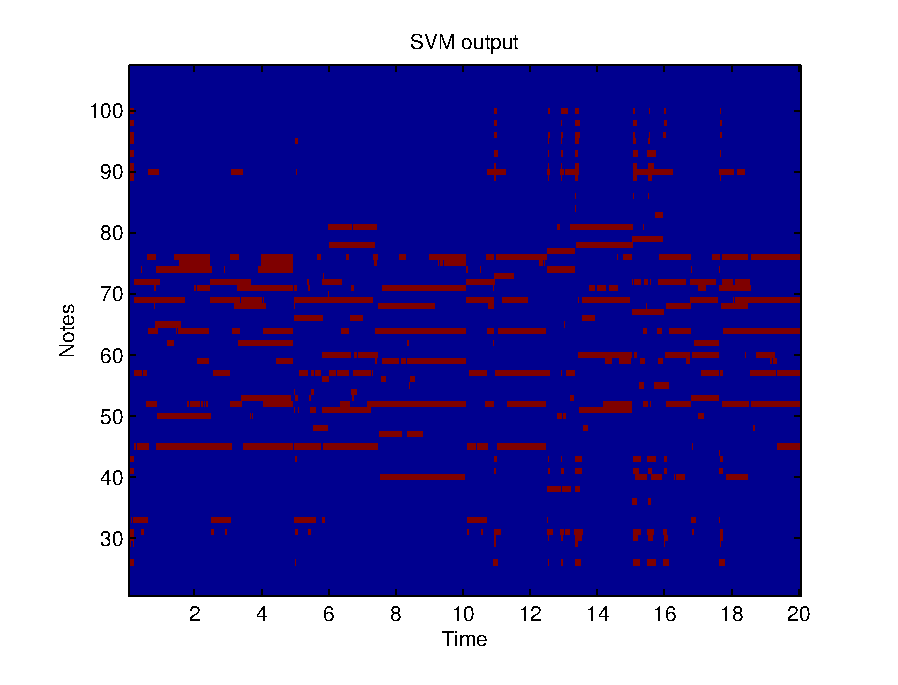
\includegraphics[scale=.6]{raw_svm}
}
\subfigure[]{
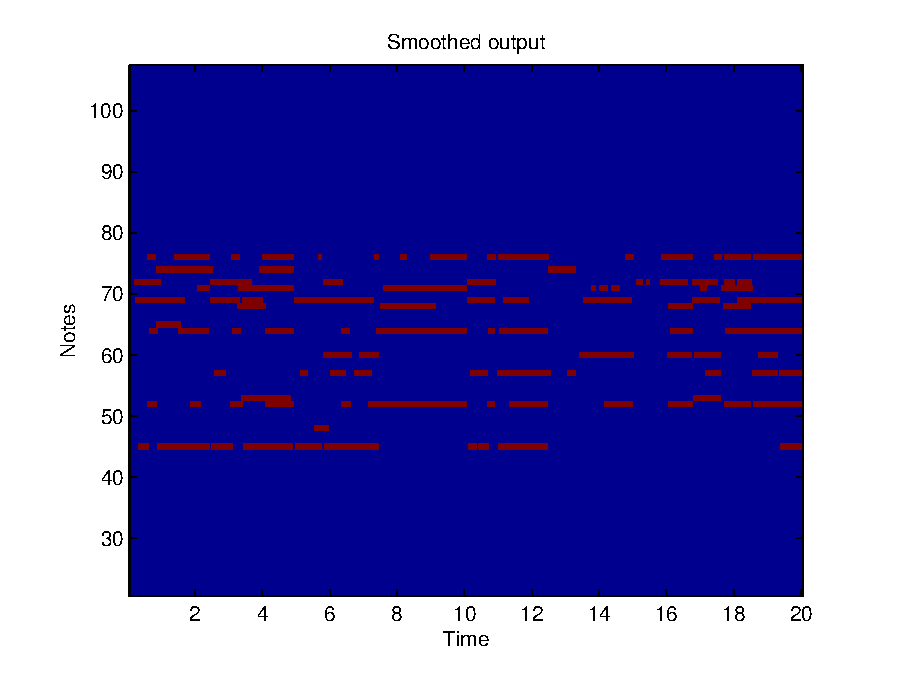
\includegraphics[scale=.6]{smoothed_svm}
}
\end{center}
\caption{ Many of the classifiers do not take temporal structure into account.  HMM smoothing captures some of this structure.  (a)  The estimated piano-roll before HMM smoothing. (b)  The estimated piano-roll after HMM smoothing}
\end{figure*}
In many of the techniques used (such as SVM's), notes at a single time step are classified independently of the notes at adjacent time steps. Since these methods do not take advantage of the temporal structure of piano music, hidden Markov models are often used for post-processing the output of the discriminative models. We model each note independently using a two-state HMM, where the states correspond to the note being on or off. The transition matrix and state priors can be estimated from the ground truth piano roll, while the emission matrix can be estimated using the output from the classifier as the observable variables. Applying the Viterbi algorithm to each note class results in a smoother piano roll that eliminates unlikely, spurious, isolated notes.

%\subsubsection{Probabilistic spectral smoothness}
%\subsection{Recurrent neural network}

\section{Evaluation}

\subsection{MIDI databases}

The MIDI music we used to evaluate these methods comes from the Classical Piano MIDI Page\footnote{http://www.piano-midi.de/}, a free, online database of piano MIDI files with a wide range of composers. This database, along with the MAPS database, are a popular choice for piano transcription researchers. Table \ref{table:songs} on page 7 gives a list of the composers and songs we used for testing and training.

The MIDI files represent the ground truth data and the training labels for our classifiers. To generate training features, we synthesized the MIDI files into WAV files using Timidity++\footnote{http://timidity.sourceforge.net/}. Since the highest fundamental frequency on a piano is 4186Hz, we chose a sampling rate of 16kHz to capture the majority of the overtone frequencies. Many researchers choose an 8kHz sampling rate to decrease the size of their input data.

\subsection{Evaluation measures}

% We use a few metrics for evaluation, as per the existing literature.

There is no standard metric to evaluate the performance of a transcription method. Researchers use a variety of error measures, described in the sections below.

\subsubsection{Overall accuracy}
$$Acc = \frac{TP}{TP+FP+FN} $$
where TP (true positives) is the number of correctly transcribed notes (over all notes), FP (false positives) is the number of unvoiced frames transcribed as voiced, and FN (false negatives) is the number of voiced frames transcribed as unvoiced. Note that notes that are missed and notes that are inserted are weighed equally.
\subsection{Frame-level transcription error score}
In the previous measure "double counts" notes transcribed correctly but at the wrong time.  Frame-level transcription error score seeks to avoid that.
At each time frame, let $N_{sys}$ be the number of reported pitches, $N_{ref}$ the ground truth number of pitches, and $N_{corr}$, their intersection, is the number of correctly reported pitches.  Then we define
$$E_{tot}=\frac{\sum_{t=1}^T \text{max}(N_{ref}(t),N_{sys}(t))-N_{corr}(t)}{\sum_{t=1}^T N_{ref}(t)}$$
$E_{tot}$ can be further split into three separate scores: $E_{sub}$, which counts the number (at each frame) of ground truth notes for which some other note was reported, $E_{miss}$, the number of ground truth notes which cannot be accounted for, and $E_{fa}$, the number of reported notes which cannot be paired with a ground truth note.  The equations for these, respectively, are
$$E_{sub}=\frac{\sum_{t=1}^T \text{min}(N_{ref}(t),N_{sys}(t))-N_{corr}(t)}{\sum_{t=1}^T N_{ref}(t)}$$
$$E_{miss}=\frac{\sum_{t=1}^T \text{max}(0,N_{ref}(t))-N_{sys}(t)}{\sum_{t=1}^T N_{ref}(t)}$$
$$E_{fa}=\frac{\sum_{t=1}^T \text{max}(0,N_{sys}(t))-N_{ref}(t)}{\sum_{t=1}^T N_{ref}(t)}$$

\subsubsection{Note Onset Detection}
Frame-level transcription error requires a high level of precision.  An error-measure perhaps more fitting for this problem is note onset detection, since onset is usually more important than offset.  To be counted as correct, our transcribed note must be turned "on" within $100$ milliseconds of the ground truth onset.
\subsection{Method comparison}

\subsubsection{Reported measures}
\begin{center}
\begin{tabular}{|l|l|l|}
\hline
Algorithm & Accuracy & $E_{tot}$ \\ \hline
SVM & 67.7\% & NR \\ \hline
SVM with HMM & 70\% & 34.2 \\ \hline
NMF & 23\% & 23 \\ \hline
Sparse NMF & 24\% & 24 \\ \hline
AdaBoost & 25\% & 25 \\ \hline
\end{tabular}
\end{center}

\subsubsection{Our evaluation}

The following table captures our evaluation of these methods. We expect these accuracy measures to be lower than they were reported in the original papers because we are using a smaller training dataset and not attempting to optimize the methods.

\begin{center}
\begin{tabular}{|l|l|l|}
\hline
Algorithm & Accuracy & $E_{tot}$ \\ \hline
SVM & 51.7\% & 84.7  \\ \hline
SVM with HMM & 62.7\% & 53.8  \\ \hline
NMF & 20\% & 20 \\ \hline
Sparse NMF & 21\% & 21 \\ \hline
AdaBoost & 22\% & 22 \\ \hline
\end{tabular}
\end{center}

\section{Conclusion}

We achieved the best results with...


% Which method is fastest

% Which method has the best performance

% Which one is the simplest method

% Future directions


\section{Individual Effort}
\begin{description}
\item[$\bullet$ Jeremy] wrote and evaluted the SVM method in \citet{poliner2006discriminative}, the non-negative matrix factorization method in \citet{abdallah2004polyphonic}, the AdaBoost method in \citet{boogaart2009note}, and wrote the paper.
\item[$\bullet$ Mark] implemented the hidden Markov model and error measures in \citet{poliner2006discriminative}, evaluated the methods, and wrote the paper.
\item[$\bullet$ Paul] implemented the non-negative matrix factorization method in \citet{abdallah2004polyphonic} and wrote the paper.
\end{description}

\begin{center}
\begin{table*}[ht]
%   \caption{Table of midi songs used for testing and training the algorithms in the paper.}
\caption{MIDI songs used for testing and training the methods in the paper.}
\begin{center}
% \setlength{\tabcolsep}{4.0em}
\begin{tabular}{L{2cm} L{4cm} L{4cm}}
% \textbf{Composer} & \textbf{Training} & \textbf{Testing} \\ \hline
Composer & Training & Testing \\ \hline
Brahms &
Sonata C major, Op. 1 (Allegro, Andante), 7 Fantasia, Op. 116 (Andante), 3 Intermezzi, Op. 117 (Andante moderato)
&
Sonata C major, Op. 1 (Finale), 7 Fantasia, Op. 116 (Andantino teneramente), 3 Intermezzi, Op. 117 (Andante moderato)
\\

Beethoven & Sonata No. 5, Op. 10 (Prestissimo), Sonata No. 8, Op. 13 (Rondo Allegro), For Elise (Poco moto) & Sonata No. 11, Op. 22 (Minuetto), Sonata No. 21, Op. 53 (Adagio molto) \\

Chopin & 5 Mazurkas, Op. 7 (Vivace), Etudes, Op. 10 (Allegro, Vivace), Etudes, Op. 25 (Allegro)
& 5 Mazurkas, Op. 7 (Vivo ma non troppo), Etudes, Op. 10 (Allegro con fuoco), Etudes, Op. 25 (Lento)
\\
Debussy & Suite bergamasque (Moderato, Menuet) & Suite bergamasque (Andante, Allegretto) \\
Mozart & Sonata No. 8 (Andantino), Sonata No. 12 (Adagio)
 & Sonata No. 8 (Allegro con spirito), Sonata No. 16 (Allegro)  \\

Schubert &
6 Moments musicaux, Op. 94 (Allegretto moderato), Fantasia C major (Presto)
& 6 Moments musicaux, Op. 94 (Allegro vivace), Fantasia C major (Allegro)
\\



% AdaBoost & 22\% & 22 \\
\end{tabular}
\end{center}
\label{table:songs}
\end{table*}
\end{center}



%    Problem statement, both conceptual and mathematical.
%    Motivation: why is the problem important.
%    Related work.
%    Methodologies explored and developed, and their advantages and disadvantages
%    Evaluation: experiments on sythetic and real data, performance measures used, results. I hope to see quantitative, objective evaluations, and comparisons with competitors
%    Conclusions: what did you learn, what were the project's success and failures?
%    Description of individual effort: At the end of the report, in a paragraph (included in the page limit), please include a brief description of each project member's contribution to the project.


% Support vector machines + HMM

% Honglak Lee's approach: use knn or RBM for input

% Non-negative matrix factorization

% Supervised NMF

% Combination NMF + svm

% Recurrent neural network (LSTM)

% Bayesian non-parametric method

% Bayesian non-parametric II (infinite hidden markov model)

% Our approach: Bayesian non parametrics with stochastic ...




%\input{1.tex}
%\input{fig1.tex}
%\input{2.tex}
%\input{3.tex}
%\input{fig2.tex}
%\input{4.tex}
%\input{5.tex}

% Your project should involve experiments that compare a few different algorithms. These should be well known or state-of-the-art methods, plus possibly any new methods you develop. The experiments should use real (as opposed to simulated) data sets. There is a large repository of machine learning data sets called the ``UCI Machine Learning Repository.'' There are other more domain-specific sources as well that you might find by searching.



%Your project should focus on a topic that has previously been studied in the machine learning literature. I include this requirement because in the past, some groups have defined entirely new problems for themselves, and been unable to make any progress.
%Your project report should contain an extensive literature review that summarizes fundamental ideas and state-of-the-art methods, with critiques of their strengths and weaknesses. My favorite reports to read are the ones that teach me something interesting.
%You are also encouraged to develop your own methods to solve your chosen problem.
%Your project should involve experiments that compare a few different algorithms. These should be well known or state-of-the-art methods, plus possibly any new methods you develop. The experiments should use real (as opposed to simulated) data sets. There is a large repository of machine learning data sets called the ``UCI Machine Learning Repository.'' There are other more domain-specific sources as well that you might find by searching.

%Every report should address the following (but don't feel obligated to make these the section headings)
%    Problem statement, both conceptual and mathematical.
%    Motivation: why is the problem important.
%    Related work.
%    Methodologies explored and developed, and their advantages and disadvantages
%    Evaluation: experiments on sythetic and real data, performance measures used, results. I hope to see quantitative, objective evaluations, and comparisons with competitors
%    Conclusions: what did you learn, what were the project's success and failures?
%    Description of individual effort: At the end of the report, in a paragraph (included in the page limit), please include a brief description of each project member's contribution to the project.


\bibliographystyle{model1-num-names}
\bibliography{transcription}
\end{document}
